\RequirePackage{luatex85}
\documentclass{standalone}
\usepackage{tikz}

% Color Definitions
\definecolor{SourceColor}{RGB}{85,168,104}
\definecolor{TargetColor}{RGB}{221,132,82}
\definecolor{TargetChangerColor}{RGB}{255,153,0}
\definecolor{AbsorbingAreaColor}{RGB}{196,78,82}
\definecolor{ObstacleColor}{RGB}{179,179,179}
\definecolor{StairColor}{RGB}{129,114,178}
\definecolor{MeasurementAreaColor}{RGB}{255,0,0}
\definecolor{InformationAreaColor}{RGB}{0,100,20}
\definecolor{AerosolCloudColor}{RGB}{202,156,76}
\definecolor{AgentColor}{RGB}{76,114,202}
\definecolor{AgentIdColor}{RGB}{255,127,0}

\newcommand{\MeasurementAreaOpacity}{0.549020}
\newcommand{\AerosolCloudOpacity}{0.039216}

\begin{document}
% Change scaling to [x=1mm,y=1mm] if TeX reports "Dimension too large".
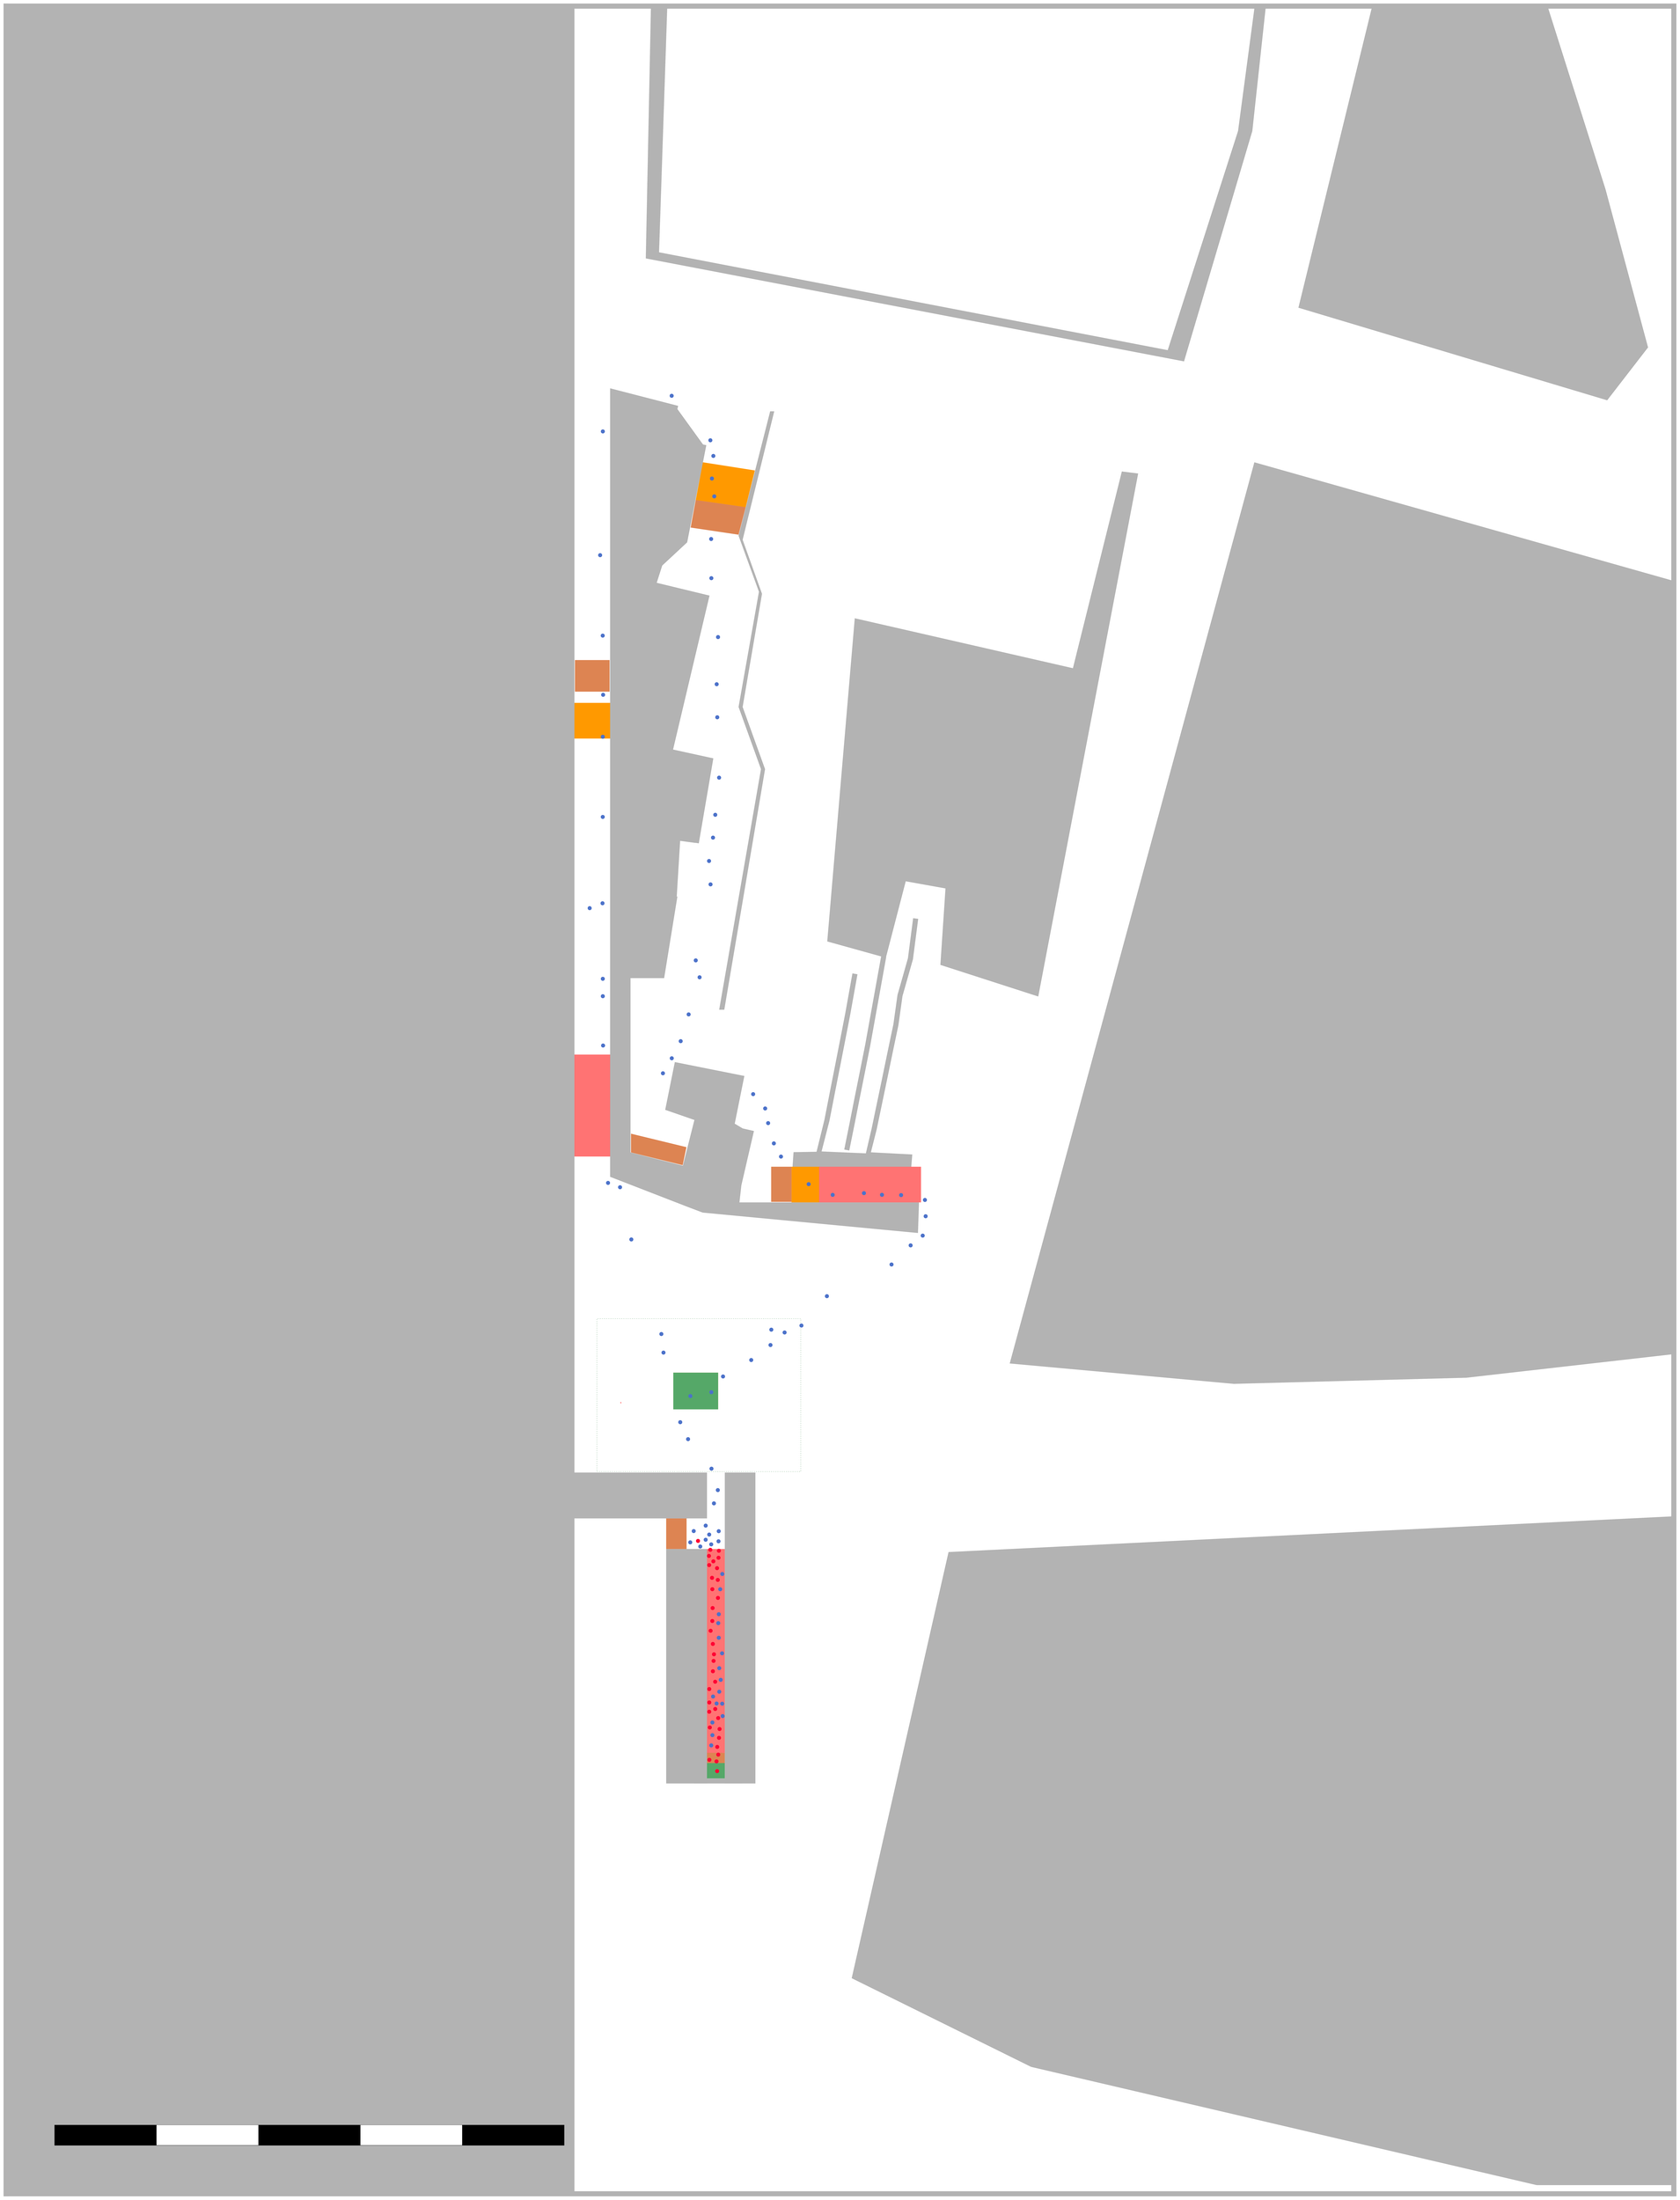
\begin{tikzpicture}
[x=1cm,y=1cm,
trajectory/.style={line width=1},
pedestrian/.style={circle, fill=AgentColor, minimum size=0.390000 cm},
walkdirection/.style={black, line width=1},
selected/.style={draw=magenta, line width=2},
group/.style={},
voronoi/.style={black, line width=1}
]
% Clipping
\clip (0.000000,0.000000) rectangle (164.100000,215.100000);
% Background
\fill[white] (0.000000,0.000000) rectangle (164.100000,215.100000);
%Information area
\draw[InformationAreaColor,opacity=1,dashed] (58.200001,71.099998) to (78.199997,71.099998) to (78.199997,86.099998) to (58.200001,86.099998) to (58.200001,71.099998);
% TargetChanger(s)
\coordinate (TargetChanger20) at (57.750000,144.750000); % Centroid: TargetChanger20
\fill[TargetChangerColor] (56.000000,143.000000) to (59.500000,143.000000) to (59.500000,146.500000) to (56.000000,146.500000) to (56.000000,143.000000);
\coordinate (TargetChanger101) at (67.900000,79.000000); % Centroid: TargetChanger101
\fill[TargetChangerColor] (65.699997,77.199997) to (70.099998,77.199997) to (70.099998,80.799995) to (65.699997,80.799995) to (65.699997,77.199997);
\coordinate (TargetChanger23) at (78.650000,99.250000); % Centroid: TargetChanger23
\fill[TargetChangerColor] (77.300003,101.000000) to (80.000000,101.000000) to (80.000000,97.500000) to (77.300003,97.500000) to (77.300003,101.000000);
\coordinate (TargetChanger202) at (70.745128,167.889231); % Centroid: TargetChanger202
\fill[TargetChangerColor] (68.599998,170.100006) to (73.699997,169.300003) to (72.800003,165.699997) to (67.900002,166.399994) to (68.599998,170.100006);
% Source(s)
\coordinate (Source4) at (69.875000,41.750000); % Centroid: Source4
\fill[SourceColor] (69.000000,41.000000) to (70.750000,41.000000) to (70.750000,42.500000) to (69.000000,42.500000) to (69.000000,41.000000);
\coordinate (Source5) at (67.900000,79.000000); % Centroid: Source5
\fill[SourceColor] (65.699997,77.199997) to (70.099998,77.199997) to (70.099998,80.799995) to (65.699997,80.799995) to (65.699997,77.199997);
% Target(s)
\coordinate (Target1000) at (64.181760,102.687914); % Centroid: Target1000
\fill[TargetColor] (66.619545,101.154007) to (61.550381,102.402931) to (61.550381,104.239578) to (66.986870,102.917191) to (66.619545,101.154007);
\coordinate (Target31) at (57.750000,149.150000); % Centroid: Target31
\fill[TargetColor] (56.049999,147.600006) to (56.049999,150.699997) to (59.450001,150.699997) to (59.450001,147.600006) to (56.049999,147.600006);
\coordinate (Target12) at (70.056203,164.708470); % Centroid: Target12
\fill[TargetColor] (72.099998,163.000000) to (67.400002,163.699997) to (67.900002,166.399994) to (72.800003,165.699997) to (72.099998,163.000000);
\coordinate (Target21) at (76.300000,99.275000); % Centroid: Target21
\fill[TargetColor] (75.300003,101.000000) to (77.300003,101.000000) to (77.300003,97.550003) to (75.300003,97.550003) to (75.300003,101.000000);
\coordinate (Target500) at (66.000000,65.000000); % Centroid: Target500
\fill[TargetColor] (65.000000,63.500000) to (67.000000,63.500000) to (67.000000,66.500000) to (65.000000,66.500000) to (65.000000,63.500000);
\coordinate (Target11) at (69.875000,43.000000); % Centroid: Target11
\fill[TargetColor] (69.000000,42.500000) to (70.750000,42.500000) to (70.750000,43.500000) to (69.000000,43.500000) to (69.000000,42.500000);
\coordinate (Target999) at (69.750000,43.000000); % Centroid: Target999
\fill[TargetColor] (69.000000,42.500000) to (70.500000,42.500000) to (70.500000,43.500000) to (69.000000,43.500000) to (69.000000,42.500000);
% AbsorbingArea(s)
% Obstacle(s)
\coordinate (Obstacle10) at (94.483203,194.457168); % Centroid: Obstacle10
\fill[ObstacleColor] (63.000000,190.100006) to (115.800003,180.000000) to (122.500000,202.600006) to (123.800003,214.600006) to (122.699997,214.600006) to (121.099998,202.600006) to (114.199997,181.100006) to (64.300003,190.699997) to (65.099998,214.600006) to (63.500000,214.600006) to (63.000000,190.100006);
\coordinate (Obstacle11) at (144.373315,195.509796); % Centroid: Obstacle11
\fill[ObstacleColor] (134.199997,214.600006) to (127.022583,185.265976) to (157.311188,176.183228) to (161.319824,181.369537) to (157.150406,196.872665) to (151.535873,214.600006) to (134.199997,214.600006);
\coordinate (Obstacle12) at (135.889014,119.655614); % Centroid: Obstacle12
\fill[ObstacleColor] (122.699997,170.100006) to (98.699997,81.699997) to (120.699997,79.699997) to (143.500000,80.300003) to (163.699997,82.599998) to (163.699997,158.500000) to (122.699997,170.100006);
\coordinate (Obstacle13) at (65.254618,135.447310); % Centroid: Obstacle13
\fill[ObstacleColor] (66.098907,175.323502) to (66.173462,175.635056) to (59.500000,177.357666) to (59.500000,100.012405) to (67.009026,97.098083) to (68.585403,96.500000) to (89.699074,94.500000) to (89.801765,97.500000) to (72.186501,97.500000) to (72.374893,99.173714) to (73.608910,104.502571) to (72.502922,104.755791) to (71.724022,105.220146) to (72.668068,109.902702) to (65.848503,111.264214) to (64.904449,106.581665) to (67.770294,105.588264) to (66.637123,101.107018) to (61.500000,102.403023) to (61.500000,119.500000) to (64.800003,119.500000) to (66.099998,127.500000) to (66.035439,127.500992) to (66.368553,132.966782) to (67.886513,132.761978) to (67.888435,132.773209) to (68.198532,132.720123) to (69.626068,141.057602) to (65.674332,141.922119) to (69.251068,157.024094) to (64.069931,158.279556) to (64.614502,159.974640) to (67.058357,162.247971) to (68.936867,171.780884) to (68.614792,171.844360) to (66.098907,175.323502);
\coordinate (Obstacle15) at (128.095228,35.558040); % Centroid: Obstacle15
\fill[ObstacleColor] (150.399994,1.100000) to (163.699997,1.100000) to (163.699997,66.699997) to (92.699997,63.200001) to (83.199997,21.400000) to (100.800003,12.700000) to (150.399994,1.100000);
\coordinate (Obstacle16) at (28.000000,107.350000); % Centroid: Obstacle16
\fill[ObstacleColor] (0.000000,0.100000) to (56.000000,0.100000) to (56.000000,214.600006) to (0.000000,214.600006) to (0.000000,0.100000);
\coordinate (Obstacle17) at (73.015628,144.617456); % Centroid: Obstacle17
\fill[ObstacleColor] (75.199997,175.100006) to (72.099998,162.899994) to (74.099998,157.399994) to (72.099998,146.100006) to (74.300003,140.000000) to (70.199997,116.400002) to (70.699997,116.400002) to (74.699997,140.000000) to (72.500000,146.100006) to (74.400002,157.199997) to (72.500000,162.500000) to (75.599998,175.100006) to (75.199997,175.100006);
\coordinate (Obstacle18) at (94.333314,138.200811); % Centroid: Obstacle18
\fill[ObstacleColor] (101.500000,117.699997) to (111.300003,169.000000) to (109.699997,169.199997) to (104.900002,149.899994) to (83.500000,154.800003) to (80.800003,123.099998) to (86.085876,121.629150) to (84.520988,112.950439) to (84.001511,110.342743) to (83.416595,107.428581) to (82.998749,105.311218) to (82.469444,102.689224) to (82.959564,102.590302) to (83.502014,105.277870) to (83.913628,107.363693) to (84.486191,110.216309) to (85.011101,112.851280) to (86.586449,121.587578) to (86.573387,121.589935) to (88.500000,129.000000) to (92.400002,128.300003) to (91.900002,120.800003) to (101.500000,117.699997);
\coordinate (Obstacle19) at (84.135704,107.887996); % Centroid: Obstacle19
\fill[ObstacleColor] (89.723122,125.313591) to (89.227310,125.378159) to (88.715431,121.447716) to (87.690865,117.843002) to (87.287964,114.963692) to (86.789063,112.596283) to (86.209267,109.791260) to (85.699806,107.350204) to (85.153625,104.733528) to (84.589127,102.310249) to (80.242821,102.497864) to (81.016670,105.513245) to (81.561340,108.305603) to (82.057617,110.816887) to (82.574249,113.456558) to (83.059326,115.950027) to (83.764503,119.875946) to (83.272377,119.964333) to (82.569641,116.050995) to (82.086319,113.566574) to (81.570740,110.932281) to (81.073174,108.414497) to (80.525436,105.606384) to (79.752518,102.466385) to (77.494728,102.427757) to (77.396767,101.000000) to (89.043594,101.000000) to (89.141563,102.200645) to (85.080162,102.412140) to (85.646210,104.646393) to (86.189262,107.248055) to (86.718216,109.782593) to (87.277489,112.488358) to (87.780586,114.875648) to (88.181374,117.739830) to (89.206390,121.346169) to (89.723122,125.313591);
\coordinate (Obstacle6) at (70.100000,40.750000); % Centroid: Obstacle6
\fill[ObstacleColor] (67.699997,40.500000) to (72.500000,40.500000) to (72.500000,41.000000) to (67.699997,41.000000) to (67.699997,40.500000);
\coordinate (Obstacle7) at (67.000000,52.000000); % Centroid: Obstacle7
\fill[ObstacleColor] (65.000000,40.500000) to (69.000000,40.500000) to (69.000000,63.500000) to (65.000000,63.500000) to (65.000000,40.500000);
\coordinate (Obstacle8) at (61.500000,68.750000); % Centroid: Obstacle8
\fill[ObstacleColor] (54.000000,66.500000) to (69.000000,66.500000) to (69.000000,71.000000) to (54.000000,71.000000) to (54.000000,66.500000);
\coordinate (Obstacle303) at (72.250000,55.750000); % Centroid: Obstacle303
\fill[ObstacleColor] (70.750000,40.500000) to (73.750000,40.500000) to (73.750000,71.000000) to (70.750000,71.000000) to (70.750000,40.500000);
% Aerosol Clouds
% Stairs
% Measurement Areas
\coordinate (MeasurementArea9) at (60.550000,77.850000); % Centroid: MeasurementArea 9
\fill[MeasurementAreaColor,opacity=\MeasurementAreaOpacity] (60.500000,77.800003) to (60.599998,77.800003) to (60.599998,77.900002) to (60.500000,77.900002) to (60.500000,77.800003);
\coordinate (MeasurementArea14) at (68.200000,78.600000); % Centroid: MeasurementArea 14

\coordinate (MeasurementArea1) at (69.875000,53.500000); % Centroid: MeasurementArea 1
\fill[MeasurementAreaColor,opacity=\MeasurementAreaOpacity] (69.000000,43.500000) to (70.750000,43.500000) to (70.750000,63.500000) to (69.000000,63.500000) to (69.000000,43.500000);
\coordinate (MeasurementArea3) at (57.750000,107.000000); % Centroid: MeasurementArea 3
\fill[MeasurementAreaColor,opacity=\MeasurementAreaOpacity] (56.000000,102.000000) to (59.500000,102.000000) to (59.500000,112.000000) to (56.000000,112.000000) to (56.000000,102.000000);
\coordinate (MeasurementArea2) at (85.000000,99.250000); % Centroid: MeasurementArea 2
\fill[MeasurementAreaColor,opacity=\MeasurementAreaOpacity] (80.000000,97.500000) to (90.000000,97.500000) to (90.000000,101.000000) to (80.000000,101.000000) to (80.000000,97.500000);
% Voronoi Diagram (not enabled in config)
% Trajectories (not enabled in config)
% Agents
\node[pedestrian] (Pedestrian309) at (64.681087,110.165441) {};
\node[pedestrian] (Pedestrian310) at (65.548006,111.637929) {};
\node[pedestrian] (Pedestrian315) at (66.423751,113.316013) {};
\node[pedestrian] (Pedestrian320) at (67.203639,115.941097) {};
\node[pedestrian] (Pedestrian326) at (68.277284,119.581838) {};
\node[pedestrian] (Pedestrian330) at (67.901497,121.239898) {};
\node[pedestrian] (Pedestrian343) at (69.352229,128.695129) {};
\node[pedestrian] (Pedestrian345) at (69.205033,130.989800) {};
\node[pedestrian] (Pedestrian350) at (69.593855,133.281049) {};
\node[pedestrian] (Pedestrian354) at (69.814829,135.520811) {};
\node[pedestrian] (Pedestrian359) at (70.190557,139.165279) {};
\node[pedestrian] (Pedestrian370) at (70.010676,145.088063) {};
\node[pedestrian] (Pedestrian375) at (69.954208,148.330865) {};
\node[pedestrian] (Pedestrian383) at (70.087256,152.955300) {};
\node[pedestrian] (Pedestrian393) at (69.431476,158.733181) {};
\node[pedestrian] (Pedestrian396) at (69.410985,162.574692) {};
\node[pedestrian] (Pedestrian405) at (69.717590,166.757165) {};
\node[pedestrian] (Pedestrian406) at (69.487354,168.507585) {};
\node[pedestrian] (Pedestrian414) at (69.626848,170.724232) {};
\node[pedestrian] (Pedestrian415) at (69.334487,172.257956) {};
\node[pedestrian] (Pedestrian423) at (70.159885,54.791722) {};
\node[pedestrian] (Pedestrian425) at (65.539024,176.623851) {};
\node[pedestrian] (Pedestrian446) at (58.786577,173.128287) {};
\node[pedestrian] (Pedestrian456) at (67.361239,64.153252) {};
\node[pedestrian] (Pedestrian466) at (58.521574,160.989391) {};
\node[pedestrian] (Pedestrian470) at (69.534792,45.238246) {};
\node[pedestrian] (Pedestrian480) at (58.775262,153.097408) {};
\node[pedestrian] (Pedestrian483) at (70.206797,49.498399) {};
\node[pedestrian] (Pedestrian485) at (70.349677,50.665027) {};
\node[pedestrian] (Pedestrian489) at (67.701318,65.258436) {};
\node[pedestrian] (Pedestrian490) at (58.813357,147.292193) {};
\node[pedestrian] (Pedestrian495) at (58.782926,143.175915) {};
\node[pedestrian] (Pedestrian505) at (75.001445,105.276546) {};
\node[pedestrian] (Pedestrian506) at (58.778989,135.312442) {};
\node[pedestrian] (Pedestrian509) at (73.531310,108.119674) {};
\node[pedestrian] (Pedestrian510) at (69.533357,46.482258) {};
\node[pedestrian] (Pedestrian514) at (74.710137,106.714308) {};
\node[pedestrian] (Pedestrian519) at (76.261774,101.993379) {};
\node[pedestrian] (Pedestrian520) at (75.563263,103.289654) {};
\node[pedestrian] (Pedestrian523) at (57.494847,126.364904) {};
\node[pedestrian] (Pedestrian524) at (58.754213,126.842767) {};
\node[pedestrian] (Pedestrian525) at (69.421073,44.233633) {};
\node[pedestrian] (Pedestrian526) at (70.541602,47.109384) {};
\node[pedestrian, fill={rgb,255: red,255; green,0; blue,51}] (Pedestrian527) at (70.169871,63.326060) {};
\node[pedestrian, fill={rgb,255: red,255; green,0; blue,51}] (Pedestrian528) at (68.123925,64.293713) {};
\node[pedestrian] (Pedestrian529) at (78.976817,99.288678) {};
\node[pedestrian] (Pedestrian530) at (69.943823,48.343409) {};
\node[pedestrian, fill={rgb,255: red,255; green,0; blue,51}] (Pedestrian531) at (69.330307,63.418835) {};
\node[pedestrian] (Pedestrian533) at (81.334138,98.236902) {};
\node[pedestrian] (Pedestrian534) at (58.783396,119.433295) {};
\node[pedestrian] (Pedestrian535) at (70.495821,48.325803) {};
\node[pedestrian] (Pedestrian536) at (58.784125,117.726605) {};
\node[pedestrian, fill={rgb,255: red,255; green,0; blue,51}] (Pedestrian537) at (69.628374,62.290870) {};
\node[pedestrian, fill={rgb,255: red,255; green,0; blue,51}] (Pedestrian538) at (69.195590,62.819092) {};
\node[pedestrian] (Pedestrian539) at (86.167522,98.242003) {};
\node[pedestrian] (Pedestrian540) at (84.401183,98.407381) {};
\node[pedestrian, fill={rgb,255: red,255; green,0; blue,51}] (Pedestrian541) at (69.989254,61.620809) {};
\node[pedestrian, fill={rgb,255: red,255; green,0; blue,51}] (Pedestrian542) at (70.135365,62.641353) {};
\node[pedestrian] (Pedestrian543) at (88.045139,98.215189) {};
\node[pedestrian] (Pedestrian544) at (69.598031,49.027703) {};
\node[pedestrian] (Pedestrian545) at (58.809621,112.888264) {};
\node[pedestrian] (Pedestrian546) at (70.205822,51.810898) {};
\node[pedestrian, fill={rgb,255: red,255; green,0; blue,51}] (Pedestrian547) at (69.218411,61.920278) {};
\node[pedestrian, fill={rgb,255: red,255; green,0; blue,51}] (Pedestrian548) at (69.528168,59.558163) {};
\node[pedestrian] (Pedestrian549) at (90.382660,97.739261) {};
\node[pedestrian] (Pedestrian550) at (70.484502,53.266357) {};
\node[pedestrian, fill={rgb,255: red,255; green,0; blue,51}] (Pedestrian551) at (70.078454,58.701283) {};
\node[pedestrian, fill={rgb,255: red,255; green,0; blue,51}] (Pedestrian552) at (69.497181,60.672119) {};
\node[pedestrian] (Pedestrian553) at (68.344801,63.744600) {};
\node[pedestrian] (Pedestrian554) at (90.453502,96.142195) {};
\node[pedestrian] (Pedestrian555) at (70.110924,56.225811) {};
\node[pedestrian] (Pedestrian556) at (90.165099,94.241564) {};
\node[pedestrian, fill={rgb,255: red,255; green,0; blue,51}] (Pedestrian557) at (69.556126,57.707069) {};
\node[pedestrian, fill={rgb,255: red,255; green,0; blue,51}] (Pedestrian558) at (70.062080,60.467344) {};
\node[pedestrian] (Pedestrian559) at (70.300199,59.551428) {};
\node[pedestrian] (Pedestrian560) at (88.980576,93.283742) {};
\node[pedestrian, fill={rgb,255: red,255; green,0; blue,51}] (Pedestrian561) at (69.524284,56.438205) {};
\node[pedestrian, fill={rgb,255: red,255; green,0; blue,51}] (Pedestrian562) at (69.359046,55.478424) {};
\node[pedestrian] (Pedestrian563) at (87.106014,91.408628) {};
\node[pedestrian] (Pedestrian564) at (70.162086,57.101886) {};
\node[pedestrian] (Pedestrian565) at (70.505421,61.048502) {};
\node[pedestrian] (Pedestrian566) at (69.418780,63.955997) {};
\node[pedestrian, fill={rgb,255: red,255; green,0; blue,51}] (Pedestrian567) at (69.577940,54.185718) {};
\node[pedestrian, fill={rgb,255: red,255; green,0; blue,51}] (Pedestrian568) at (69.689118,53.172699) {};
\node[pedestrian] (Pedestrian569) at (59.296011,99.411166) {};
\node[pedestrian] (Pedestrian570) at (60.474810,98.986829) {};
\node[pedestrian, fill={rgb,255: red,255; green,0; blue,51}] (Pedestrian571) at (69.228231,48.444130) {};
\node[pedestrian, fill={rgb,255: red,255; green,0; blue,51}] (Pedestrian572) at (69.648530,52.522422) {};
\node[pedestrian] (Pedestrian573) at (70.134028,64.255440) {};
\node[pedestrian] (Pedestrian574) at (68.873519,64.407197) {};
\node[pedestrian] (Pedestrian575) at (69.219893,64.916360) {};
\node[pedestrian] (Pedestrian576) at (80.766848,88.300836) {};
\node[pedestrian, fill={rgb,255: red,255; green,0; blue,51}] (Pedestrian577) at (69.806054,50.477311) {};
\node[pedestrian, fill={rgb,255: red,255; green,0; blue,51}] (Pedestrian578) at (69.582572,51.506405) {};
\node[pedestrian] (Pedestrian579) at (61.580593,93.865610) {};
\node[pedestrian] (Pedestrian580) at (70.155505,65.246773) {};
\node[pedestrian, fill={rgb,255: red,255; green,0; blue,51}] (Pedestrian581) at (69.810883,47.806872) {};
\node[pedestrian, fill={rgb,255: red,255; green,0; blue,51}] (Pedestrian582) at (69.227713,49.761879) {};
\node[pedestrian] (Pedestrian583) at (68.875959,65.792302) {};
\node[pedestrian] (Pedestrian584) at (78.267672,85.420069) {};
\node[pedestrian] (Pedestrian585) at (75.312709,85.014862) {};
\node[pedestrian] (Pedestrian586) at (76.616503,84.739522) {};
\node[pedestrian, fill={rgb,255: red,255; green,0; blue,51}] (Pedestrian587) at (70.101279,46.915120) {};
\node[pedestrian, fill={rgb,255: red,255; green,0; blue,51}] (Pedestrian588) at (69.224566,47.534962) {};
\node[pedestrian] (Pedestrian589) at (69.684756,67.976576) {};
\node[pedestrian] (Pedestrian590) at (75.232552,83.508045) {};
\node[pedestrian, fill={rgb,255: red,255; green,0; blue,51}] (Pedestrian591) at (69.281190,45.993071) {};
\node[pedestrian, fill={rgb,255: red,255; green,0; blue,51}] (Pedestrian592) at (70.236426,45.839868) {};
\node[pedestrian] (Pedestrian593) at (73.342795,82.036328) {};
\node[pedestrian] (Pedestrian594) at (70.067118,69.277491) {};
\node[pedestrian] (Pedestrian595) at (69.444178,71.378622) {};
\node[pedestrian] (Pedestrian596) at (64.527357,84.588296) {};
\node[pedestrian, fill={rgb,255: red,255; green,0; blue,51}] (Pedestrian597) at (70.008475,44.083178) {};
\node[pedestrian, fill={rgb,255: red,255; green,0; blue,51}] (Pedestrian598) at (70.180386,44.976724) {};
\node[pedestrian] (Pedestrian599) at (64.735557,82.765086) {};
\node[pedestrian] (Pedestrian600) at (70.578084,80.423362) {};
\node[pedestrian, fill={rgb,255: red,255; green,0; blue,51}] (Pedestrian601) at (70.109238,43.328668) {};
\node[pedestrian, fill={rgb,255: red,255; green,0; blue,51}] (Pedestrian602) at (69.936926,42.666885) {};
\node[pedestrian] (Pedestrian603) at (67.147469,74.276305) {};
\node[pedestrian] (Pedestrian604) at (69.429492,78.883343) {};
\node[pedestrian] (Pedestrian605) at (66.380301,75.938850) {};
\node[pedestrian] (Pedestrian606) at (67.371313,78.501420) {};
\node[pedestrian, fill={rgb,255: red,255; green,0; blue,51}] (Pedestrian607) at (69.998501,41.709830) {};
\node[pedestrian, fill={rgb,255: red,255; green,0; blue,51}] (Pedestrian608) at (69.237412,42.819097) {};
\node[pedestrian] (Pedestrian309) at (64.681087,110.165441) {};
\node[pedestrian] (Pedestrian310) at (65.548006,111.637929) {};
\node[pedestrian] (Pedestrian315) at (66.423751,113.316013) {};
\node[pedestrian] (Pedestrian320) at (67.203639,115.941097) {};
\node[pedestrian] (Pedestrian326) at (68.277284,119.581838) {};
\node[pedestrian] (Pedestrian330) at (67.901497,121.239898) {};
\node[pedestrian] (Pedestrian343) at (69.352229,128.695129) {};
\node[pedestrian] (Pedestrian345) at (69.205033,130.989800) {};
\node[pedestrian] (Pedestrian350) at (69.593855,133.281049) {};
\node[pedestrian] (Pedestrian354) at (69.814829,135.520811) {};
\node[pedestrian] (Pedestrian359) at (70.190557,139.165279) {};
\node[pedestrian] (Pedestrian370) at (70.010676,145.088063) {};
\node[pedestrian] (Pedestrian375) at (69.954208,148.330865) {};
\node[pedestrian] (Pedestrian383) at (70.087256,152.955300) {};
\node[pedestrian] (Pedestrian393) at (69.431476,158.733181) {};
\node[pedestrian] (Pedestrian396) at (69.410985,162.574692) {};
\node[pedestrian] (Pedestrian405) at (69.717590,166.757165) {};
\node[pedestrian] (Pedestrian406) at (69.487354,168.507585) {};
\node[pedestrian] (Pedestrian414) at (69.626848,170.724232) {};
\node[pedestrian] (Pedestrian415) at (69.334487,172.257956) {};
\node[pedestrian] (Pedestrian423) at (70.159885,54.791722) {};
\node[pedestrian] (Pedestrian425) at (65.539024,176.623851) {};
\node[pedestrian] (Pedestrian446) at (58.786577,173.128287) {};
\node[pedestrian] (Pedestrian456) at (67.361239,64.153252) {};
\node[pedestrian] (Pedestrian466) at (58.521574,160.989391) {};
\node[pedestrian] (Pedestrian470) at (69.534792,45.238246) {};
\node[pedestrian] (Pedestrian480) at (58.775262,153.097408) {};
\node[pedestrian] (Pedestrian483) at (70.206797,49.498399) {};
\node[pedestrian] (Pedestrian485) at (70.349677,50.665027) {};
\node[pedestrian] (Pedestrian489) at (67.701318,65.258436) {};
\node[pedestrian] (Pedestrian490) at (58.813357,147.292193) {};
\node[pedestrian] (Pedestrian495) at (58.782926,143.175915) {};
\node[pedestrian] (Pedestrian505) at (75.001445,105.276546) {};
\node[pedestrian] (Pedestrian506) at (58.778989,135.312442) {};
\node[pedestrian] (Pedestrian509) at (73.531310,108.119674) {};
\node[pedestrian] (Pedestrian510) at (69.533357,46.482258) {};
\node[pedestrian] (Pedestrian514) at (74.710137,106.714308) {};
\node[pedestrian] (Pedestrian519) at (76.261774,101.993379) {};
\node[pedestrian] (Pedestrian520) at (75.563263,103.289654) {};
\node[pedestrian] (Pedestrian523) at (57.494847,126.364904) {};
\node[pedestrian] (Pedestrian524) at (58.754213,126.842767) {};
\node[pedestrian] (Pedestrian525) at (69.421073,44.233633) {};
\node[pedestrian] (Pedestrian526) at (70.541602,47.109384) {};
\node[pedestrian, fill={rgb,255: red,255; green,0; blue,51}] (Pedestrian527) at (70.169871,63.326060) {};
\node[pedestrian, fill={rgb,255: red,255; green,0; blue,51}] (Pedestrian528) at (68.123925,64.293713) {};
\node[pedestrian] (Pedestrian529) at (78.976817,99.288678) {};
\node[pedestrian] (Pedestrian530) at (69.943823,48.343409) {};
\node[pedestrian, fill={rgb,255: red,255; green,0; blue,51}] (Pedestrian531) at (69.330307,63.418835) {};
\node[pedestrian] (Pedestrian533) at (81.334138,98.236902) {};
\node[pedestrian] (Pedestrian534) at (58.783396,119.433295) {};
\node[pedestrian] (Pedestrian535) at (70.495821,48.325803) {};
\node[pedestrian] (Pedestrian536) at (58.784125,117.726605) {};
\node[pedestrian, fill={rgb,255: red,255; green,0; blue,51}] (Pedestrian537) at (69.628374,62.290870) {};
\node[pedestrian, fill={rgb,255: red,255; green,0; blue,51}] (Pedestrian538) at (69.195590,62.819092) {};
\node[pedestrian] (Pedestrian539) at (86.167522,98.242003) {};
\node[pedestrian] (Pedestrian540) at (84.401183,98.407381) {};
\node[pedestrian, fill={rgb,255: red,255; green,0; blue,51}] (Pedestrian541) at (69.989254,61.620809) {};
\node[pedestrian, fill={rgb,255: red,255; green,0; blue,51}] (Pedestrian542) at (70.135365,62.641353) {};
\node[pedestrian] (Pedestrian543) at (88.045139,98.215189) {};
\node[pedestrian] (Pedestrian544) at (69.598031,49.027703) {};
\node[pedestrian] (Pedestrian545) at (58.809621,112.888264) {};
\node[pedestrian] (Pedestrian546) at (70.205822,51.810898) {};
\node[pedestrian, fill={rgb,255: red,255; green,0; blue,51}] (Pedestrian547) at (69.218411,61.920278) {};
\node[pedestrian, fill={rgb,255: red,255; green,0; blue,51}] (Pedestrian548) at (69.528168,59.558163) {};
\node[pedestrian] (Pedestrian549) at (90.382660,97.739261) {};
\node[pedestrian] (Pedestrian550) at (70.484502,53.266357) {};
\node[pedestrian, fill={rgb,255: red,255; green,0; blue,51}] (Pedestrian551) at (70.078454,58.701283) {};
\node[pedestrian, fill={rgb,255: red,255; green,0; blue,51}] (Pedestrian552) at (69.497181,60.672119) {};
\node[pedestrian] (Pedestrian553) at (68.344801,63.744600) {};
\node[pedestrian] (Pedestrian554) at (90.453502,96.142195) {};
\node[pedestrian] (Pedestrian555) at (70.110924,56.225811) {};
\node[pedestrian] (Pedestrian556) at (90.165099,94.241564) {};
\node[pedestrian, fill={rgb,255: red,255; green,0; blue,51}] (Pedestrian557) at (69.556126,57.707069) {};
\node[pedestrian, fill={rgb,255: red,255; green,0; blue,51}] (Pedestrian558) at (70.062080,60.467344) {};
\node[pedestrian] (Pedestrian559) at (70.300199,59.551428) {};
\node[pedestrian] (Pedestrian560) at (88.980576,93.283742) {};
\node[pedestrian, fill={rgb,255: red,255; green,0; blue,51}] (Pedestrian561) at (69.524284,56.438205) {};
\node[pedestrian, fill={rgb,255: red,255; green,0; blue,51}] (Pedestrian562) at (69.359046,55.478424) {};
\node[pedestrian] (Pedestrian563) at (87.106014,91.408628) {};
\node[pedestrian] (Pedestrian564) at (70.162086,57.101886) {};
\node[pedestrian] (Pedestrian565) at (70.505421,61.048502) {};
\node[pedestrian] (Pedestrian566) at (69.418780,63.955997) {};
\node[pedestrian, fill={rgb,255: red,255; green,0; blue,51}] (Pedestrian567) at (69.577940,54.185718) {};
\node[pedestrian, fill={rgb,255: red,255; green,0; blue,51}] (Pedestrian568) at (69.689118,53.172699) {};
\node[pedestrian] (Pedestrian569) at (59.296011,99.411166) {};
\node[pedestrian] (Pedestrian570) at (60.474810,98.986829) {};
\node[pedestrian, fill={rgb,255: red,255; green,0; blue,51}] (Pedestrian571) at (69.228231,48.444130) {};
\node[pedestrian, fill={rgb,255: red,255; green,0; blue,51}] (Pedestrian572) at (69.648530,52.522422) {};
\node[pedestrian] (Pedestrian573) at (70.134028,64.255440) {};
\node[pedestrian] (Pedestrian574) at (68.873519,64.407197) {};
\node[pedestrian] (Pedestrian575) at (69.219893,64.916360) {};
\node[pedestrian] (Pedestrian576) at (80.766848,88.300836) {};
\node[pedestrian, fill={rgb,255: red,255; green,0; blue,51}] (Pedestrian577) at (69.806054,50.477311) {};
\node[pedestrian, fill={rgb,255: red,255; green,0; blue,51}] (Pedestrian578) at (69.582572,51.506405) {};
\node[pedestrian] (Pedestrian579) at (61.580593,93.865610) {};
\node[pedestrian] (Pedestrian580) at (70.155505,65.246773) {};
\node[pedestrian, fill={rgb,255: red,255; green,0; blue,51}] (Pedestrian581) at (69.810883,47.806872) {};
\node[pedestrian, fill={rgb,255: red,255; green,0; blue,51}] (Pedestrian582) at (69.227713,49.761879) {};
\node[pedestrian] (Pedestrian583) at (68.875959,65.792302) {};
\node[pedestrian] (Pedestrian584) at (78.267672,85.420069) {};
\node[pedestrian] (Pedestrian585) at (75.312709,85.014862) {};
\node[pedestrian] (Pedestrian586) at (76.616503,84.739522) {};
\node[pedestrian, fill={rgb,255: red,255; green,0; blue,51}] (Pedestrian587) at (70.101279,46.915120) {};
\node[pedestrian, fill={rgb,255: red,255; green,0; blue,51}] (Pedestrian588) at (69.224566,47.534962) {};
\node[pedestrian] (Pedestrian589) at (69.684756,67.976576) {};
\node[pedestrian] (Pedestrian590) at (75.232552,83.508045) {};
\node[pedestrian, fill={rgb,255: red,255; green,0; blue,51}] (Pedestrian591) at (69.281190,45.993071) {};
\node[pedestrian, fill={rgb,255: red,255; green,0; blue,51}] (Pedestrian592) at (70.236426,45.839868) {};
\node[pedestrian] (Pedestrian593) at (73.342795,82.036328) {};
\node[pedestrian] (Pedestrian594) at (70.067118,69.277491) {};
\node[pedestrian] (Pedestrian595) at (69.444178,71.378622) {};
\node[pedestrian] (Pedestrian596) at (64.527357,84.588296) {};
\node[pedestrian, fill={rgb,255: red,255; green,0; blue,51}] (Pedestrian597) at (70.008475,44.083178) {};
\node[pedestrian, fill={rgb,255: red,255; green,0; blue,51}] (Pedestrian598) at (70.180386,44.976724) {};
\node[pedestrian] (Pedestrian599) at (64.735557,82.765086) {};
\node[pedestrian] (Pedestrian600) at (70.578084,80.423362) {};
\node[pedestrian, fill={rgb,255: red,255; green,0; blue,51}] (Pedestrian601) at (70.109238,43.328668) {};
\node[pedestrian, fill={rgb,255: red,255; green,0; blue,51}] (Pedestrian602) at (69.936926,42.666885) {};
\node[pedestrian] (Pedestrian603) at (67.147469,74.276305) {};
\node[pedestrian] (Pedestrian604) at (69.429492,78.883343) {};
\node[pedestrian] (Pedestrian605) at (66.380301,75.938850) {};
\node[pedestrian] (Pedestrian606) at (67.371313,78.501420) {};
\node[pedestrian, fill={rgb,255: red,255; green,0; blue,51}] (Pedestrian607) at (69.998501,41.709830) {};
\node[pedestrian, fill={rgb,255: red,255; green,0; blue,51}] (Pedestrian608) at (69.237412,42.819097) {};
% Agent Ids (not enabled in config)
% Topography Boundary
\coordinate (TopographyBoundary1) at (82.050000,0.250000); % Centroid: TopographyBoundary -1
\fill[ObstacleColor] (-0.000100,0.500100) to (-0.000100,-0.000100) to (164.100098,-0.000100) to (164.100098,0.500100) to (-0.000100,0.500100);
\coordinate (TopographyBoundary2) at (163.850000,107.550000); % Centroid: TopographyBoundary -1
\fill[ObstacleColor] (163.599899,-0.000100) to (164.100098,-0.000100) to (164.100098,215.100098) to (163.599899,215.100098) to (163.599899,-0.000100);
\coordinate (TopographyBoundary3) at (82.050000,214.850000); % Centroid: TopographyBoundary -1
\fill[ObstacleColor] (164.100098,214.599899) to (164.100098,215.100098) to (-0.000100,215.100098) to (-0.000100,214.599899) to (164.100098,214.599899);
\coordinate (TopographyBoundary4) at (0.250000,107.550000); % Centroid: TopographyBoundary -1
\fill[ObstacleColor] (0.500100,215.100098) to (-0.000100,215.100098) to (-0.000100,-0.000100) to (0.500100,-0.000100) to (0.500100,215.100098);

\draw[fill=black] (5,5) rectangle ++(10,2);
\draw[fill=white] (15,5) rectangle ++(10,2);
\draw[fill=black] (25,5) rectangle ++(10,2);
\draw[fill=white] (35,5) rectangle ++(10,2);
\draw[fill=black] (45,5) rectangle ++(10,2);



\end{tikzpicture}
\end{document}
